\documentclass[a4paper]{article}

\usepackage{fullpage} % Package to use full page
\usepackage{parskip} % Package to tweak paragraph skipping
\usepackage{tikz} % Package for drawing
\usepackage{amsmath}
\usepackage{hyperref}
\usepackage[T1]{fontenc}
\usepackage{tabto}
\usepackage{subfig}
\usepackage{booktabs}
\usepackage{float}

\title{EECS 542 (Computer Vision) - HW1 \\ Convolutional Neural Networks}
\author{Yash Bhalgat (Uniqname: yashsb)}
\date{September 24, 2017}
\begin{document}

\maketitle

\section{Part 1}
Codes for the following layers written and checked: \\
\textit{Convolution, Pooling, Linear, Leaky\_ReLU, Batch Normalization, softmax and loss\_crossentropy}.

Batch normalization backprop equations taken from \cite{bn}.

**Results and plots shown together in Part 2

\section{Part 2}

In this part, I trained and tested the network over the MNIST dataset. Apart from a basic baseline model, the effects of using leaky ReLU and batch-normalization are also reflected.

\subsection{Baseline model for the CNN}

\subsubsection{Baseline Model}
\fbox{\begin{minipage}{\linewidth}
Input size -> [28,28,1]\\
Layer 1 output size -> [24,24,8] \tab    ...\{Conv layer\}\\
Layer 2 output size -> [11,11,8] \tab    ...\{Max Pooling layer\}\\
Layer 3 output size -> [11,11,8] \tab    ...\{ReLU activation\}\\
Layer 4 output size -> 968       \tab    ...\{Flatten\}\\
Layer 5 output size -> 10        \tab    ...\{Linear layer\}\\
Layer 6 output size -> 10        \tab    ...\{Softmax layer\}
\end{minipage}}


\textbf{Decisions and Reasoning}:
\begin{enumerate}
    \item A filter size of 3x3 to 7x7 is appropriate to extract the features. After some tuning, 5x5 turned out to be the best filter size.
    \item To keep the higher order features intact, I chose a pooling grid of size 4x4 with a stride of 2 (so overlapping windows).
    \item I could use multiple (two) fully connected layers. But there was no significant increase by adding a linear layer. Hence the linear layer size was chosen to map the features from 968-dim to 10-dim
    \item Softmax layer is used at the end to output a set of probabilities for each class to choose the maximum as the prediction
\end{enumerate}

\subsubsection{Hyper parameters of the network}
In this assignment, the test set is used as the validation set. Hence, all the hyper parameters are tuned over the test set. The best performance is obtained by choosing the following params:\\
\fbox{\begin{minipage}{15em}
batch\_size -> 100\\
lr (learning rate) -> 0.2\\
wd (weight decay) -> 0.0004
\end{minipage}}


\subsubsection{Baseline model: Explanation and results}
Choosing a smaller batch size implies larger time for each epoch. So, a batch size smaller than 100 did not seem appropriate. Also, a batch size like 1000 gave a 2\% dip in the accuracy. While training, each batch was randomly chosen from the training set and passed through the network. The following figures show the performance of the network in terms of training losses, testing losses and accuracy.\\

% \begin{verbatim}
% def illustrate(f, a):
%     """
%     Function to take a function and illustrate the limiting definition of a derivative at a given point.
%     """
%     lst = []
%     for h in srange(.01, 3, .01):
%     	lst.append([h,(f(a+h)-f(a))/h])
%     return list_plot(lst, axes_labels=['$x$','$\\frac{f(%.02f+h)-f(%.02f)}{h}$' % (a,a)])
% \end{verbatim}
\begin{figure}[htb]
	\centering
	\subfloat[]{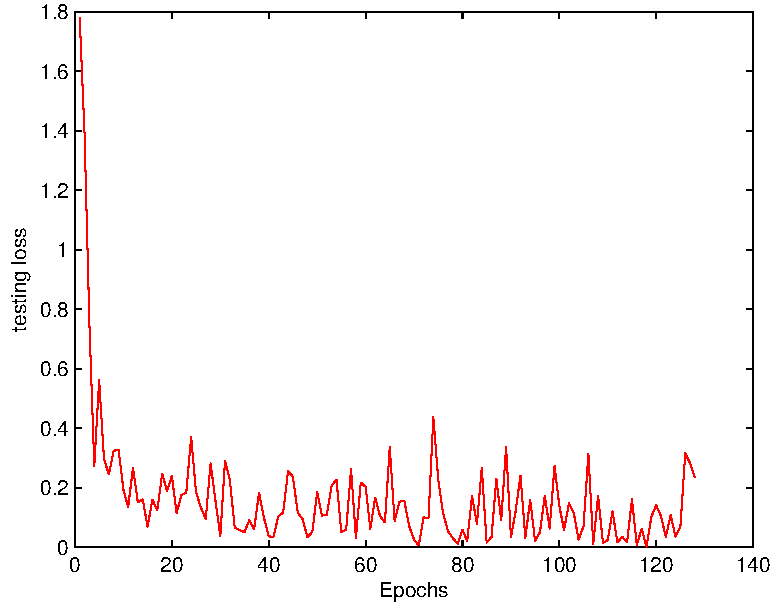
\includegraphics[width=0.45\linewidth]{figures/training_loss_baseline.pdf}}\hfill
	\subfloat[]{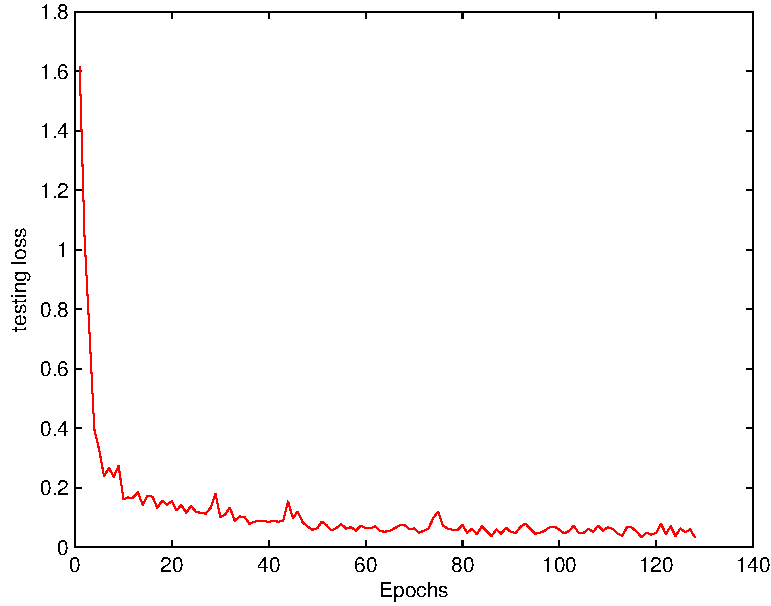
\includegraphics[width=0.45\linewidth]{figures/testing_loss_baseline.pdf}}\hfill
	\caption{Training and testing loss across epochs \label{fig:1}}
\end{figure}

\begin{figure}[htb]
	\centering
	\includegraphics[width=0.6\linewidth]{figures/testing_accuracy_baseline.pdf}
	\caption{Testing accuracy for the \textbf{Baseline Model} across epochs \label{fig:2}}
\end{figure}

The maximum accuracy is achieved at 128 epochs (10 iters per epoch).The model reached a maximum test-accuracy of \textbf{99.38\%}, which greater than the required 96\% accuracy in the assignment. 

\vspace{-10pt}

\section{Effects of Batch-normalization layer and Leaky-ReLU}
\vspace{-5pt}
According to \cite{bn}, the batch normalization significantly reduces training time and gives a jump in accuracy especially in very deep networks. So, to test the effect of the BN layer, I ran the problem through a new network - just by adding a BN layer after the convolution layer.

\fbox{\begin{minipage}{\linewidth}
\textbf{New network with BN layer}:\\
Input size -> [28,28,1]\\
Layer 1 output size -> [24,24,8] \tab    ...\{Conv layer\}\\
Layer 2 output size -> [11,11,8] \tab    ...\{Max Pooling layer\}\\
Layer 3 output size -> [11,11,8] \tab    ...\{Batch Norm layer\}\\   
Layer 3 output size -> [11,11,8] \tab    ...\{ReLU activation\}\\
Layer 4 output size -> 968       \tab    ...\{Flatten\}\\
Layer 5 output size -> 10        \tab    ...\{Linear layer\}\\
Layer 6 output size -> 10        \tab    ...\{Softmax layer\}
\end{minipage}}

As another part of testing, I replaced all the ReLU activations by leaky-ReLU functions. After running through the network while keeping the hyper parameters same, following results were obtained:

\begin{table}[!htb]
\begin{center}
\begin{tabular}{cccc}
\toprule
\multicolumn{1}{c}{} & \multicolumn{1}{c}{Baseline} & \multicolumn{1}{c}{Batch-Norm} & \multicolumn{1}{c}{leaky-ReLU}\\
\midrule
Accuracy after 1280 iters (\%) & \textbf{99.38} & 97.45 & 98.82\\
Train loss after 1280 iters & 0.2339 & 0.3368 & \textbf{0.2247}\\
Test loss after 1280 iters & \textbf{0.0337} & 0.0984 & 0.0891\\
\# of iters to reach 96\% accuracy & 350 & 280 & \textbf{220}\\
\bottomrule
\end{tabular}
\caption{Results and comparison of different methods for feature extraction \label{table:1}}
\end{center}\end{table}
\vspace{-5pt}

It can be observed that Batch normalization doesn't give any advantage, mainly because the network is not very deep and we already have a high accuracy. And the leaky-ReLU is helpful only in reducing the # of training epochs required to reach a destination accuracy.

\begin{figure}[H]
	\centering
	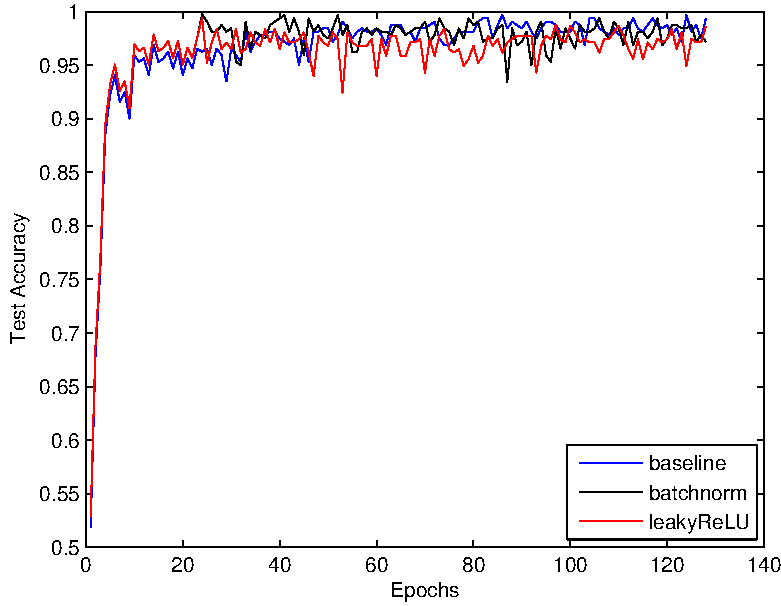
\includegraphics[width=0.7\linewidth]{figures/comparison_accuracy.pdf}
	\caption{Comparison of test accuracy through different models \label{fig:4}}
\end{figure}

\begin{figure}[H]
	\centering
	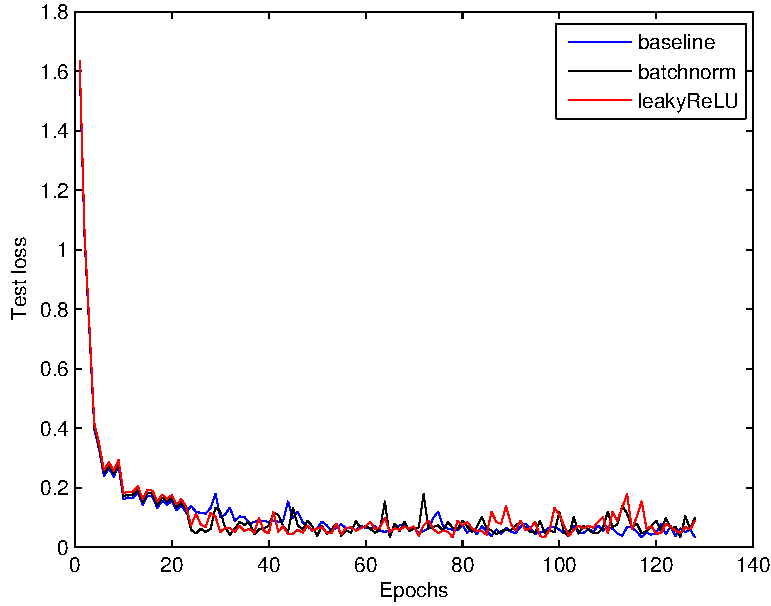
\includegraphics[width=0.7\linewidth]{figures/comparison_testloss.pdf}
	\caption{Comparison of testing/validation loss through different models \label{fig:5}}
\end{figure}

\begin{figure}[H]
	\centering
	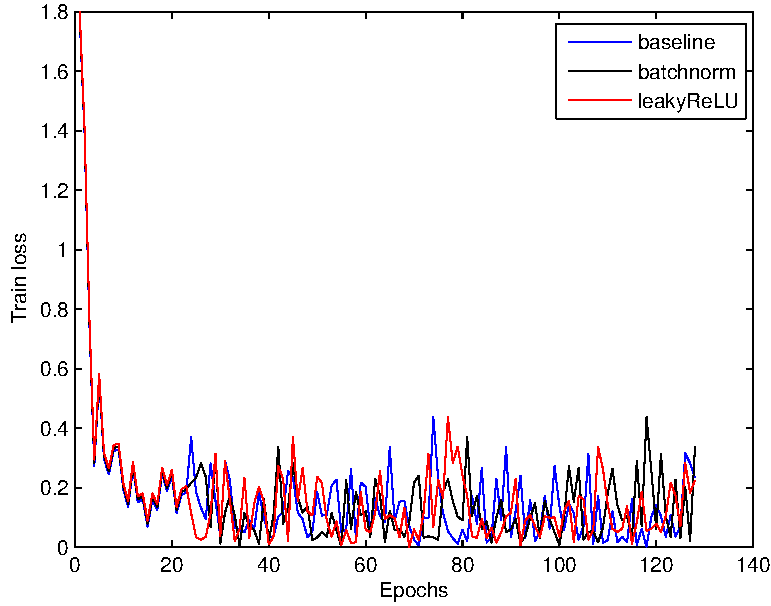
\includegraphics[width=0.7\linewidth]{figures/comparison_trainloss.pdf}
	\caption{Comparison of training loss through different models \label{fig:6}}
\end{figure}



\bibliographystyle{plain}
\bibliography{bibliography.bib}
\end{document}